\documentclass{article}
\usepackage[utf8]{inputenc}
\usepackage{amsmath}
\usepackage{amsthm}
\usepackage{bm}
\usepackage{amsfonts}
\usepackage{titlesec}
\usepackage{hyperref}
\usepackage{color}
\usepackage{booktabs}
\usepackage{amsthm}
\usepackage{listings}
\usepackage{exsheets}

%% Font Policy
% vector, \bm{}
% matrix, \bm{}
% space, \mathbb{}

%%%% Define "Lecture" (from redefining "Chapter") %%%% 
% \titleformat{\chapter}[block]{\LARGE\bfseries}{Lecture~\arabic{chapter}.}{1em}{}[]
%%%% ============================================ %%%%

%%% Set up exercise-solution format %%%
%\SetupExSheets{
	%	counter-format = ch.qu ,
	%	counter-within = chapter
	%}
%%% =============================== %%%

\renewcommand{\vec}[1]{\bm{#1}}
\newtheorem*{remark}{Remark}
\newtheorem{theorem}{Theorem}[section]
\newtheorem{definition}{Definition}[section]
\newtheorem{problem}{Problem}
\newtheorem{corollary}{Corollary}[section]
\newtheorem{lemma}{Lemma}[section]
\newtheorem{property}{Property}[section]

\author{Fang Zhu}
\title{Lecture 6 Projectors}

\begin{document}
	\maketitle
	
\section{Prerequisite}


\section{Solutions}
\subsection{Exercise 6.1}
\begin{proof}
    Since $\bm{P}$ is an orthogonal projector, then we have $\bm{P}^2 = \bm{P}$ and $\bm{P}^{\star} = \bm{P}$, hence 
    \begin{equation}
        (\bm{I} - 2\bm{P})^{\star}  (\bm{I} - 2\bm{P}) = \bm{I} - 2\bm{P}^\star - 2 \bm{P} + 4 \bm{P}^\star \bm{P} = 0,
    \end{equation}
    which means that $\bm{I} - 2 \bm{P}$ is unitary. A geometric interpretation is given by \autoref{fig:geo_e61}.
    \begin{figure}[htpb]
        \centering
        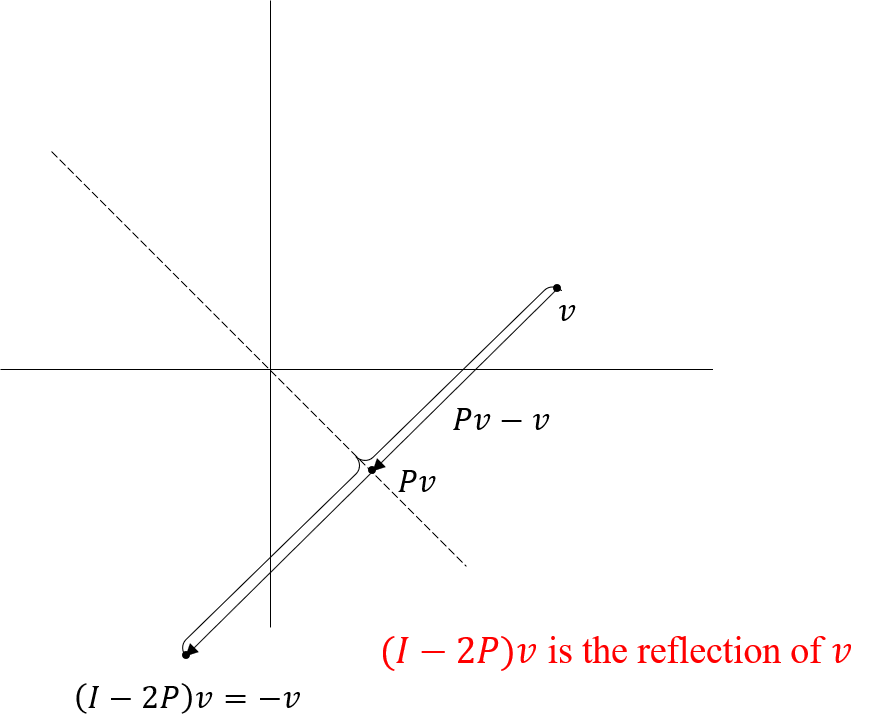
\includegraphics[width=0.5\textwidth]{e61.png}
        \caption{Geometric interpretation of $\bm{I} - 2\bm{P}$.}
        \label{fig:geo_e61}
    \end{figure}
\end{proof}

\subsection{Exercise 6.2}
We begin by considering the matrix \(\bm{F}\) defined by
\[
\bm{F} =
\begin{pmatrix}
	0 & \cdots & 0 & 1 \\
	0 & \cdots & 1 & 0 \\
	\vdots & \ddots & \vdots & \vdots \\
	1 & \cdots & 0 & 0
\end{pmatrix},
\]
where \(\bm{F}\) is a permutation matrix that reverses the order of the basis vectors. Consequently, we define
\[
\bm{E} = \frac{\bm{I} + \bm{F}}{2} = 
\begin{pmatrix}
	\frac{1}{2} & 0 & \cdots & 0 & \frac{1}{2} \\
	0 & \frac{1}{2} & \cdots & \frac{1}{2} & 0 \\
	\vdots & \vdots & \ddots & \vdots & \vdots \\
	0 & \cdots & 1 & \cdots & 0 \\
	\vdots & \vdots & \vdots & \ddots & \vdots \\
	\frac{1}{2} & \cdots & 0 & 0 & \frac{1}{2}
\end{pmatrix},
\]
where \(\bm{I}\) is the identity matrix. Observing that \(\bm{F}\) is its own inverse, i.e., \(\bm{F}^2 = \bm{I}\), and that the adjoint of a matrix is equal to its conjugate transpose, we deduce that the adjoint of \(\bm{E}\), denoted \(\bm{E}^\star\), satisfies
\[
\bm{E}^\star = \left(\frac{\bm{I} + \bm{F}}{2}\right)^\star = \bm{E},
\]
since both \(\bm{I}\) and \(\bm{F}\) are real and symmetric, and thus equal to their own adjoints.

Next, we compute \(\bm{E}^2\) as follows:
\[
\bm{E}^2 = \left(\frac{\bm{I} + \bm{F}}{2}\right)^2 = \frac{\bm{I} + 2\bm{F} + \bm{F}^2}{4} = \frac{2\bm{I} + 2\bm{F}}{4} = \frac{\bm{I} + \bm{F}}{2} = \bm{E}.
\]
Hence, \(\bm{E}^2 = \bm{E}\), which implies that \(\bm{E}\) is idempotent. Additionally, since for any vector \(\bm{v}\), the equality \(\langle \bm{E}\bm{v}, \bm{v} \rangle = \langle \bm{v}, \bm{E}\bm{v} \rangle\) holds, where \(\langle \cdot, \cdot \rangle\) denotes the inner product, it follows that \(\bm{E}\) is self-adjoint. Combining the idempotence and self-adjointness of \(\bm{E}\), we conclude that \(\bm{E}\) is an orthogonal projector.

\subsection{Exercise 5.3}

Suppose that $\bm{A}$ is full rank. This implies that $\bm{A}$ has $n$ non-zero singular values. Consequently, the matrix $\bm{A}^\star \bm{A}$, where $\bm{A}^\star$ denotes the conjugate transpose of $\bm{A}$, has $n$ non-zero eigenvalues $\lambda_1, \ldots, \lambda_n$. The determinant of $\bm{A}^\star \bm{A}$ is then given by the product of its eigenvalues:
\[
\det(\bm{A}^\star \bm{A}) = \prod_{i=1}^n \lambda_i \neq 0,
\]
which indicates that $\bm{A}^\star \bm{A}$ is non-singular.

For the ``only if'' part of the proof, we invoke the singular value decomposition (SVD). Since $\bm{A}^\star \bm{A}$ is non-singular, it follows from Theorem 5.2 that
\[
\mathrm{range}(\bm{A}) = \langle \bm{u}_1, \ldots, \bm{u}_n \rangle,
\]
where the $\bm{u}_i$ are left singular vectors of $\bm{A}^\star \bm{A}$. This space is $n$-dimensional, which confirms that the matrix $\bm{A}$ is indeed full rank.


\subsection{Exercise 6.4 (a) }
We first compute $\bm{P}$ as 
$$
\bm{P} = \bm{A} (\bm{A}^\star \bm{A} )^{-1} \bm{A}^\star = 
\begin{pmatrix}
	\frac{1}{2} & 0 & \frac{1}{2}\\
	0 & 1 & 0 \\
	\frac{1}{2} & 0 & \frac{1}{2}
\end{pmatrix} 
$$
then 
$$
\bm{P} \begin{pmatrix}
	1 \\
	2\\
	3
\end{pmatrix} = \begin{pmatrix}
2 \\
2\\
2
\end{pmatrix}.
$$

\subsection{Exercise 6.4(b) }
We first compute $\bm{P}$ as 
$$
\bm{P} = \bm{B} (\bm{B}^\star \bm{B} )^{-1} \bm{B}^\star = 
\begin{pmatrix}
	\frac{5}{6} & \frac{1}{3} & \frac{1}{6}\\
	\frac{1}{3} & \frac{1}{3} &-\frac{1}{3} \\
	\frac{1}{6} & -\frac{1}{3} & \frac{5}{6}
\end{pmatrix} 
$$
then 
$$
\bm{P} \begin{pmatrix}
	1 \\
	2\\
	3
\end{pmatrix} = \begin{pmatrix}
	2 \\
	0\\
	2
\end{pmatrix}.
$$

\subsection{Exercise 6.5}
The solution is based on the answer on \href{https://math.stackexchange.com/questions/1109755/a-projection-p-is-orthogonal-if-and-only-if-its-spectral-norm-is-1}{Mathematics Stack Exchange}. We first show that $\| \bm{P} \|_2 \geq 1$. Choose $\bm{x}$ such that $ \bm{Px} = \bm{y} \neq \bm{0}$, then $ \bm{P} \bm{y} = \bm{P}^2 \bm{x} = \bm{P} \bm{x} = \bm{y}$, then we have
$$
\| \bm{P} \|_2 = \max_{\bm{x} }  \frac{\| \bm{P x} \|_2}{ \| \bm{x} \|_2 } \geq \frac{\| \bm{P y} \|_2}{ \| \bm{y} \|_2 } = 1.
$$
Assume that $\bm{P} $ is orthogonal projector, then we have that
$$
\bm {P}  = \hat{\bm{Q}} \hat{\bm{Q}}^{\star}
$$
where the columns of $\hat{\bm{Q}}$ are orthonormal. Hence we can get that
$$
1\leq \| \bm{P} \|_2 \leq \|\hat{\bm{Q}} \|_2 \| \hat{\bm{Q}}^{\star}\|_2 \leq 1
$$
which means that $\| \bm{P} \|_2 = 1$. If $\| \bm{P} \| = 1$, we only to show that $\mathrm{range}(\bm{P})  \perp \mathrm{null} (\bm{P})$. Let $\bm{x}$ be a vector such that $\bm{x} \in \mathrm{null} (\bm{P})^{\perp} $ and consider $ \bm{y} := \bm{Px} - \bm{x} $. It is clear that $\bm{y} \in \mathrm{null} (\bm{P}) $, then $\bm{x} \perp \bm{y} $. Since $\| \bm{P}\|_2 = 1$, we have $\| \bm{Px}\|_2 \leq \| \bm{x} \|_2 $. It follows that
$$
 \| \bm{x} \|_2 \leq \| \bm{x} \|_2 + \|\bm{y} \|_2 = \| \bm{x} + \bm{y} \|_2 = \| \bm{Px}\|_2 \leq \| \bm{x} \|_2
$$
and hence $\bm{y} = \bm{0}$, which implies that $\| \bm{Px} \|_2 = \| \bm{x} \|_2$ and thus $\bm{x} \in \mathrm{range} (\bm{P}) $. Therefore $\mathrm{null} (\bm{P})^{\perp} \subset \mathrm{range} (\bm{P}) $. On the other hand, if $\bm{z} \in \mathrm{range} (\bm{P}), \bm{Pz} = \bm{z} $, Let $\bm{x} \in \mathrm{null} (\bm{P}) $ and $\bm{y} \in  \mathrm{null} (\bm{P})^\perp$ such that $\bm{z} = \bm{x} + \bm{y}$, so $\bm{Pz} = \bm{Px} + \bm{Py}  = \bm{Py}$. Since $\mathrm{null} (\bm{P})^\perp \subset \mathrm{range} (\bm{P}) $, we have $\bm{Py} = \bm{y} $ and $\bm{y} = \bm{z} $ and $\bm{z} \in \mathrm{null} (\bm{P})^\perp $. Therefore $\mathrm{range} (\bm{P}) \subset \mathrm{null} (\bm{P})^\perp$. From $\mathrm{range} (\bm{P}) \subset \mathrm{null} (\bm{P})^\perp $ and $\mathrm{range} (\bm{P}) \supset \mathrm{null} (\bm{P})^\perp$, it follows that $\mathrm{range} (\bm{P}) = \mathrm{null} (\bm{P})^\perp$.
\end{document}